\hypertarget{product_8inc}{
\section{include/product.inc File Reference}
\label{product_8inc}\index{include/product.inc@{include/product.inc}}
}
Functions to output Product Info. 

\subsection*{Functions}
\begin{CompactItemize}
\item 
\hyperlink{product_8inc_9dbb778854cfe105058d7161ca8f058c}{getImages} (\$product)
\end{CompactItemize}


\subsection{Detailed Description}
Functions to output Product Info. 

Various pieces of info gleamed from the web will be handled by functions contained in this file. Currently, it only handles getting product images 

Definition in file \hyperlink{product_8inc-source}{product.inc}.

\subsection{Function Documentation}
\hypertarget{product_8inc_9dbb778854cfe105058d7161ca8f058c}{
\index{product.inc@{product.inc}!getImages@{getImages}}
\index{getImages@{getImages}!product.inc@{product.inc}}
\subsubsection{\setlength{\rightskip}{0pt plus 5cm}getImages (\$ {\em product})}}
\label{product_8inc_9dbb778854cfe105058d7161ca8f058c}


Gets Appropriate Images from google Image Search \begin{Desc}
\item[Parameters:]
\begin{description}
\item[{\em \$product}]The product to get images for \end{description}
\end{Desc}
\begin{Desc}
\item[Returns:]HTML code to output product images \end{Desc}
\begin{Desc}
\item[\hyperlink{todo__todo000001}{Todo}]Make images more accurate 

Add left and right arrows to choose image to show \end{Desc}


Definition at line 17 of file product.inc.

References fget().

Referenced by getBarcodeInfo().

\begin{Code}\begin{verbatim}17                              {
21   $json = json_decode(fget('http://ajax.googleapis.com/ajax/services/search/images?v=1.0&q=' . urlencode($product)));
25   $imgpath = $json->responseData->results[0]->tbUrl;
29   $imgsource = $json->responseData->results[0]->visibleUrl;
33   $imgsourceurl = $json->responseData->results[0]->tbUrl;
37   $imgcontext = $json->responseData->results[0]->originalContextUrl;
41   $output = '';
42   $output = <<<_HTML
43     <div id="prodimg">
44       <a href="$imgcontext" target="_blank">
45         <img src="$imgpath" alt="Image of $product From $imgsource" title="Image of $product From $imgsource">
46       </a><br />
47       <a href="aboutimages.html" target="_blank" onclick="popup(this.href, 200, 300); return false;">About this image</a>
48     </div>
49 _HTML;
50 
51   return $output;
52 }
\end{verbatim}
\end{Code}




Here is the call graph for this function:\nopagebreak
\begin{figure}[H]
\begin{center}
\leavevmode
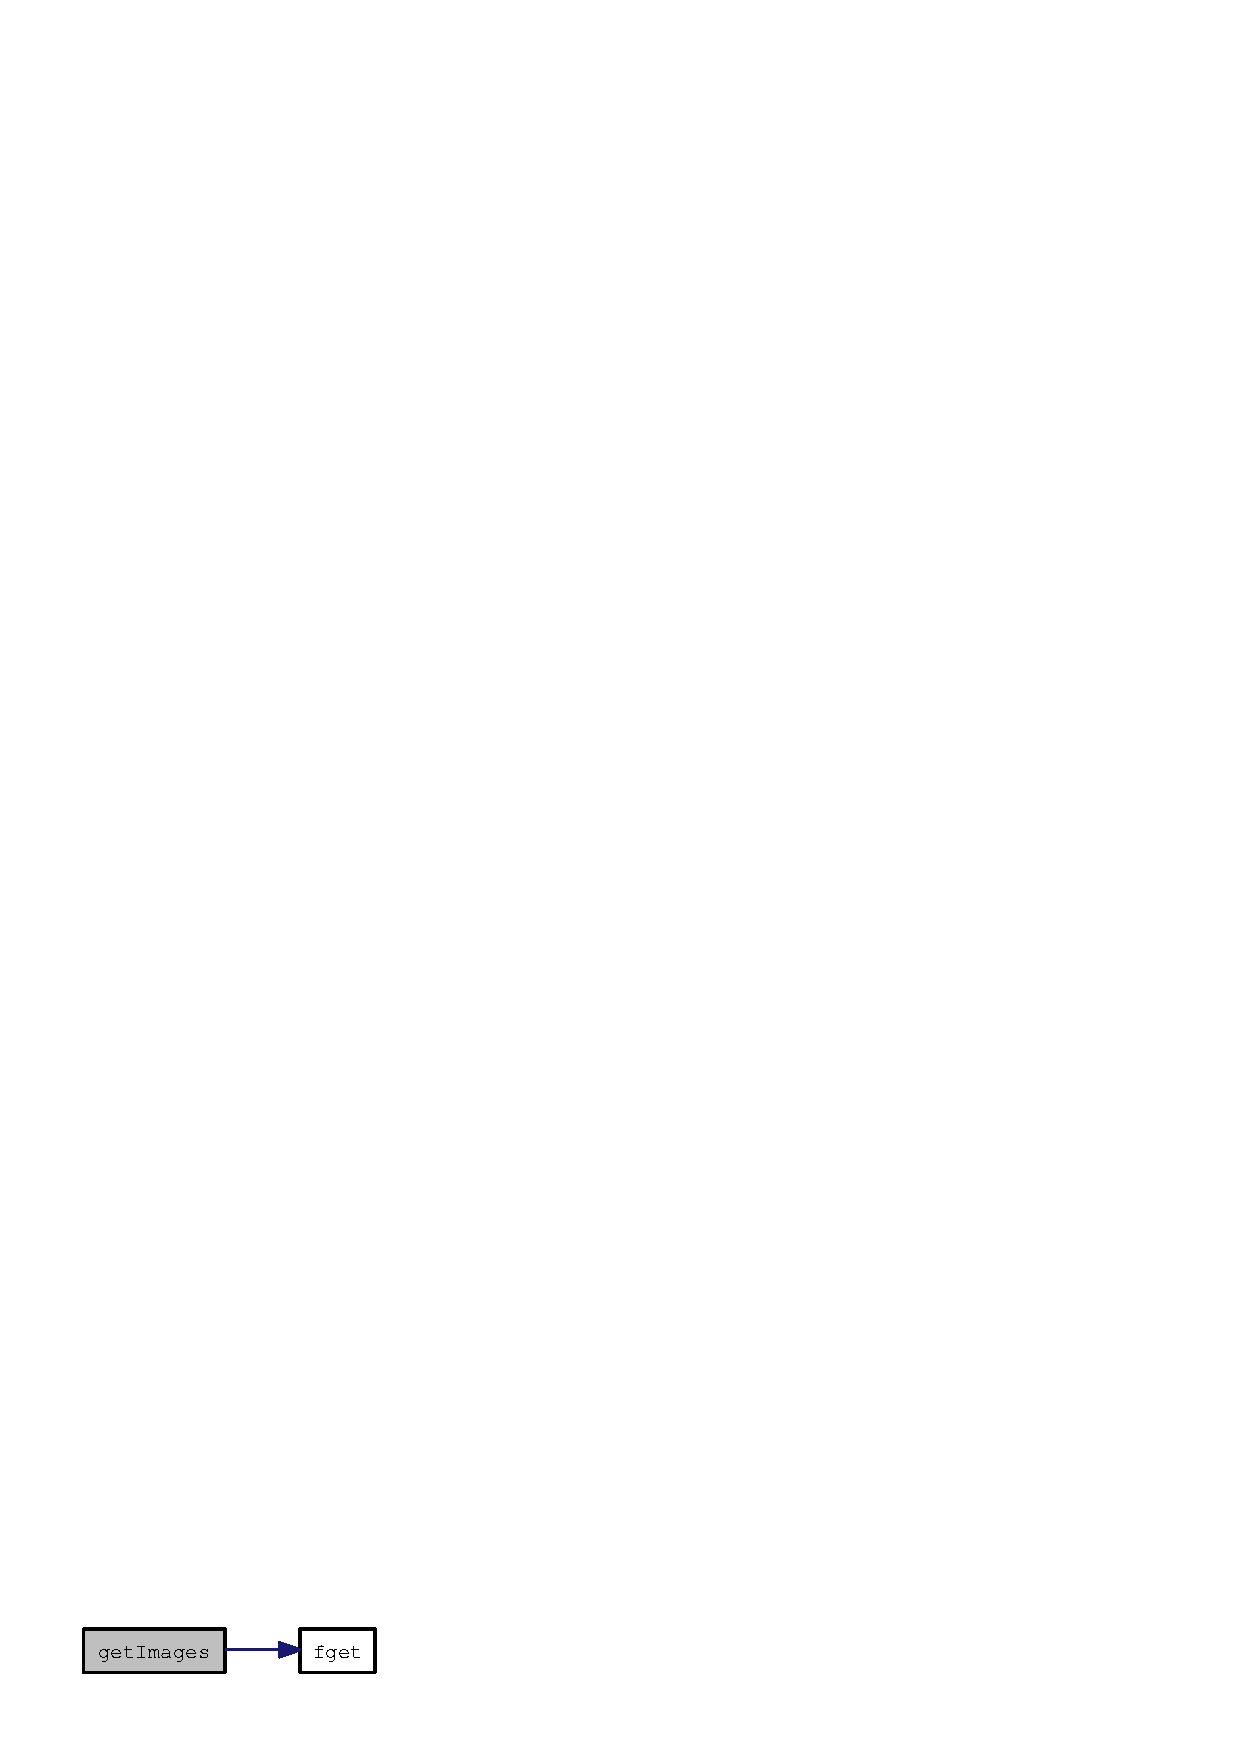
\includegraphics[width=92pt]{product_8inc_9dbb778854cfe105058d7161ca8f058c_cgraph}
\end{center}
\end{figure}


Here is the caller graph for this function:\nopagebreak
\begin{figure}[H]
\begin{center}
\leavevmode
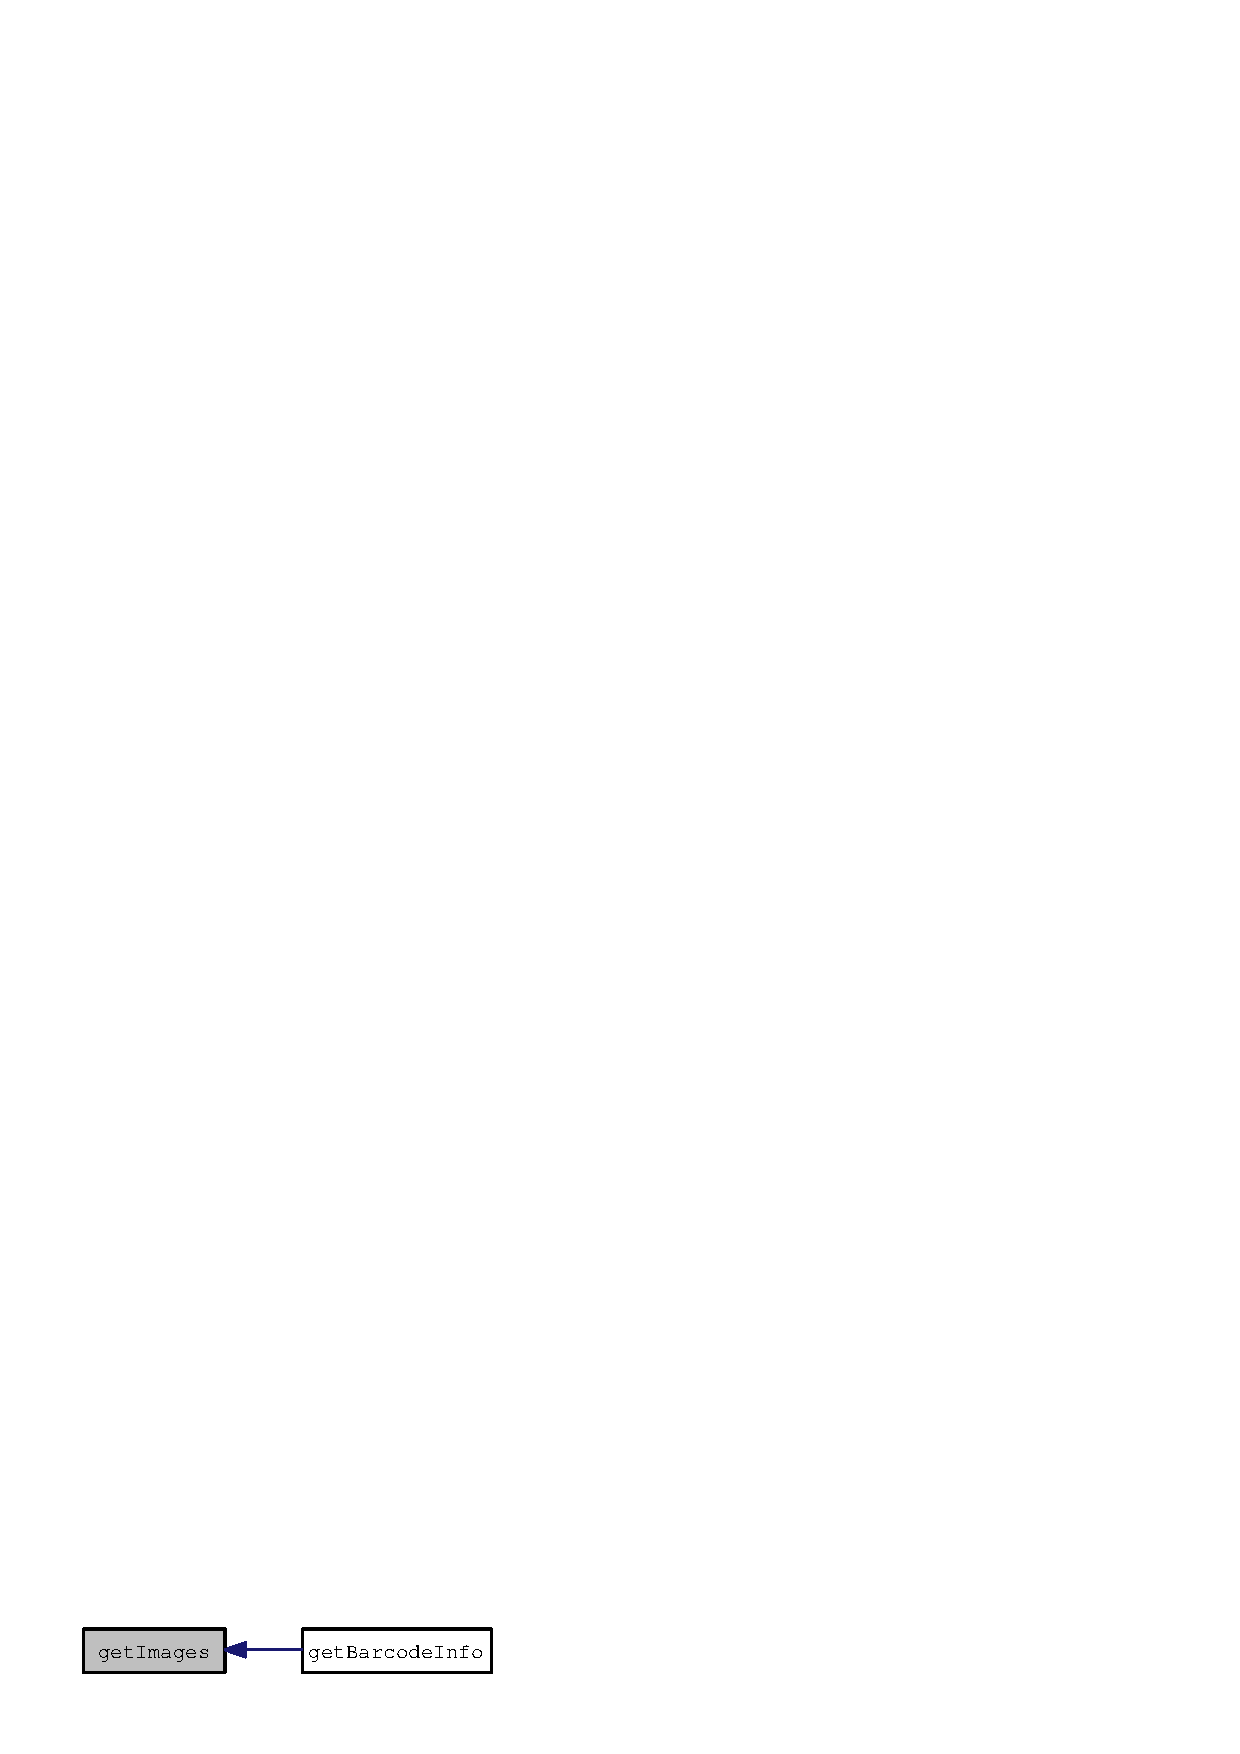
\includegraphics[width=120pt]{product_8inc_9dbb778854cfe105058d7161ca8f058c_icgraph}
\end{center}
\end{figure}
